\section{Results}\label{sec:results}
\GenMainTable

\paragraph{Main comparison.} Table~\ref{tab:main} and Fig.~\ref{fig:main} give the results; Fig.~\ref{fig:examples} shows examples. On all three datasets the learned encoder beats every causal baseline on SSIM, low-pass SSIM and PSNR, and uses less charge than the calibrated intensity baseline:
\begin{itemize}
\item \textbf{Letters.} Low-pass SSIM is \NumLettersLearnLp\ against \NumLettersIntLp. Accuracy is \NumLettersLearnAcc\ against \NumLettersIntAcc, which is on par with the same classifier on the original images (\NumLettersCeil).
\item \textbf{MNIST.} Every reasonable encoder gets near the ceiling (\NumMnistLearnAcc\ against \NumMnistIntAcc, ceiling \NumMnistCeil), so 1024 well-spread sites carry digits easily. Image fidelity still separates the encoders: low-pass SSIM is \NumMnistLearnLp\ against \NumMnistIntLp.
\item \textbf{CIFAR-10.} The ceiling is low because grayscale 32\,px objects are hard even unprosthetised (\NumCifarCeil). The learned encoder raises accuracy from \NumCifarIntAcc\ to \NumCifarLearnAcc\ and low-pass SSIM from \NumCifarIntLp\ to \NumCifarLearnLp.
\item \textbf{Charge.} The learned encoder uses \NumMnistLearnCharge\ against \NumMnistIntCharge\,\textmu C of summed charge per phase on MNIST, and \NumLettersLearnCharge\ against \NumLettersIntCharge\ on letters.
\end{itemize}
The two edge-based encoders score poorly on image similarity by construction, since they render outlines of filled shapes. They are also below intensity sampling on recognition here. Scene simplification aimed at navigation \citep{han2021deep} needs semantic segmentation, which our light saliency proxy does not provide.

\paragraph{Amortised versus per-image optimisation.} Per-image optimisation knows the true patient and optimises each frame separately, evaluated on the first 128 test images per patient. On MNIST and letters it is only marginally better than the single-pass learned encoder (SSIM \NumMnistOracleSsim\ against \NumMnistLearnSsim; \NumLettersOracleSsim\ against \NumLettersLearnSsim). On CIFAR it is clearly better (\NumCifarOracleSsim\ against \NumCifarLearnSsim), which leaves headroom for larger encoders on natural images. It also stimulates fewer electrodes (\NumMnistOracleActive\ against \NumMnistLearnActive\ on MNIST). With 100 Adam steps through the fast renderer it is a reference point, not an upper bound.

\paragraph{Patient adaptation.} Fine-tuning only the per-electrode gain and bias on a patient's calibrated forward model raised SSIM on every dataset:
\begin{itemize}
\item MNIST: \NumMnistLearnSsim\,$\to$\,\NumMnistAdaptSsim;
\item letters: \NumLettersLearnSsim\,$\to$\,\NumLettersAdaptSsim;
\item CIFAR: \NumCifarLearnSsim\,$\to$\,\NumCifarAdaptSsim;
\item CIFAR low-pass SSIM: \NumCifarLearnLp\,$\to$\,\NumCifarAdaptLp.
\end{itemize}
Recognition changed little: MNIST \NumMnistLearnAcc\,$\to$\,\NumMnistAdaptAcc, letters \NumLettersLearnAcc\,$\to$\,\NumLettersAdaptAcc, CIFAR \NumCifarLearnAcc\,$\to$\,\NumCifarAdaptAcc. The generic encoder knows neither thresholds nor dead electrodes, and only \NumMnistLearnSupraPct\% of the currents it delivers on MNIST exceed the patient's detection threshold. Calibrated intensity sampling puts \NumMnistIntSupraPct\% above threshold. The adapter did not raise this share (\NumMnistAdaptSupraPct\%). Instead it used more of the active-electrode budget (\NumMnistAdaptActive\ against \NumMnistLearnActive\ active electrodes) at a lower median current (\NumMnistAdaptMedAmp\ against \NumMnistLearnMedAmp\,\textmu A), i.e.\ more but dimmer and smaller phosphenes. Figure~\ref{fig:adapt} shows how the gain depends on the number of unlabeled images (MNIST, two patients). Sixteen images give no reliable gain (\NumShotAdptA\ SSIM). The adapter's gain grows to \NumShotAdptD\ with 1024 images, while full fine-tuning at the same step budget levels off near \NumShotFullC. At this step budget, restricting adaptation to the per-electrode parameters is both cheaper and more effective.

\begin{figure*}[t]
\centering
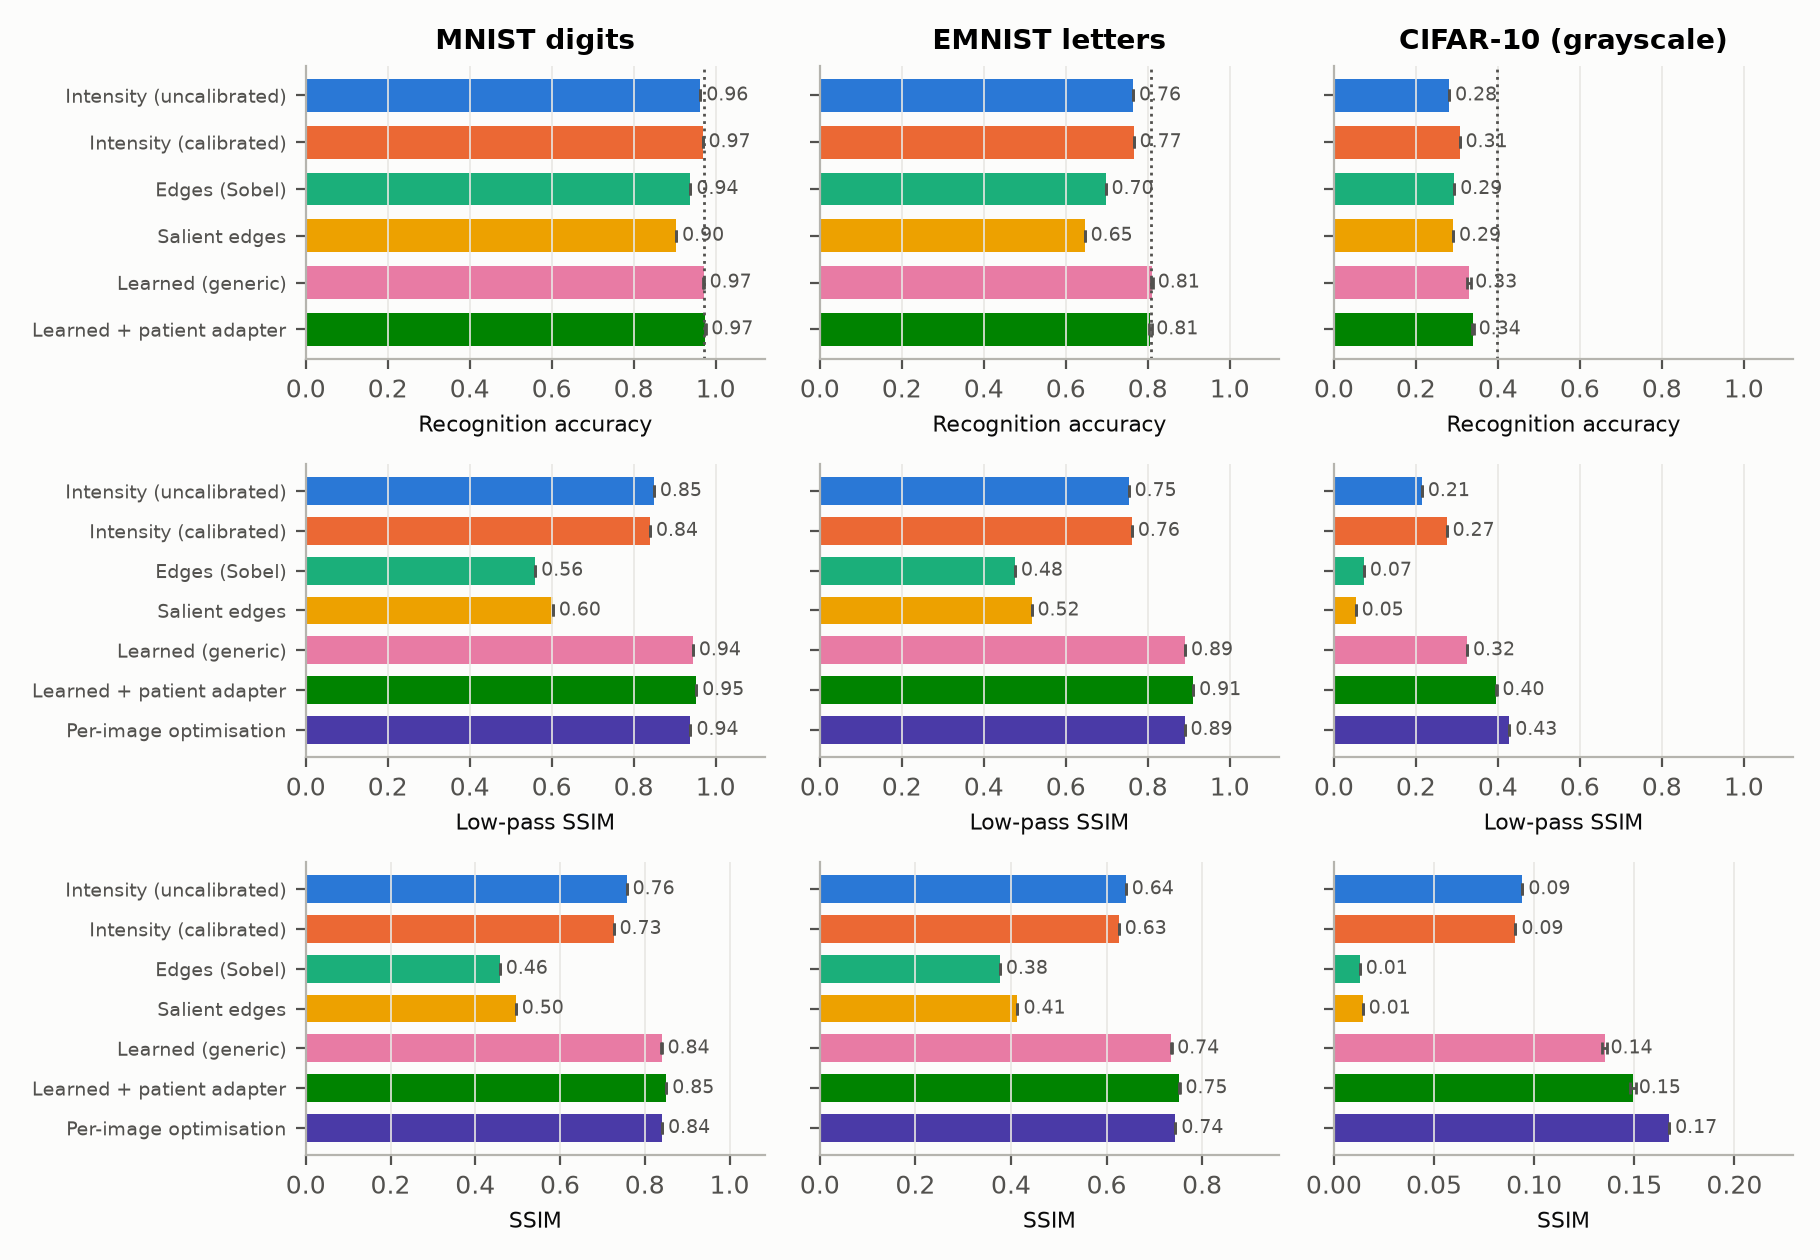
\includegraphics[width=\textwidth]{fig_main_results.png}
\caption{Main results per dataset (five held-out patients; learned rows show mean and s.d.\ over three training seeds). The dotted line marks the classifier's accuracy on the original images.}
\label{fig:main}
\end{figure*}

\begin{figure}[t]
\centering
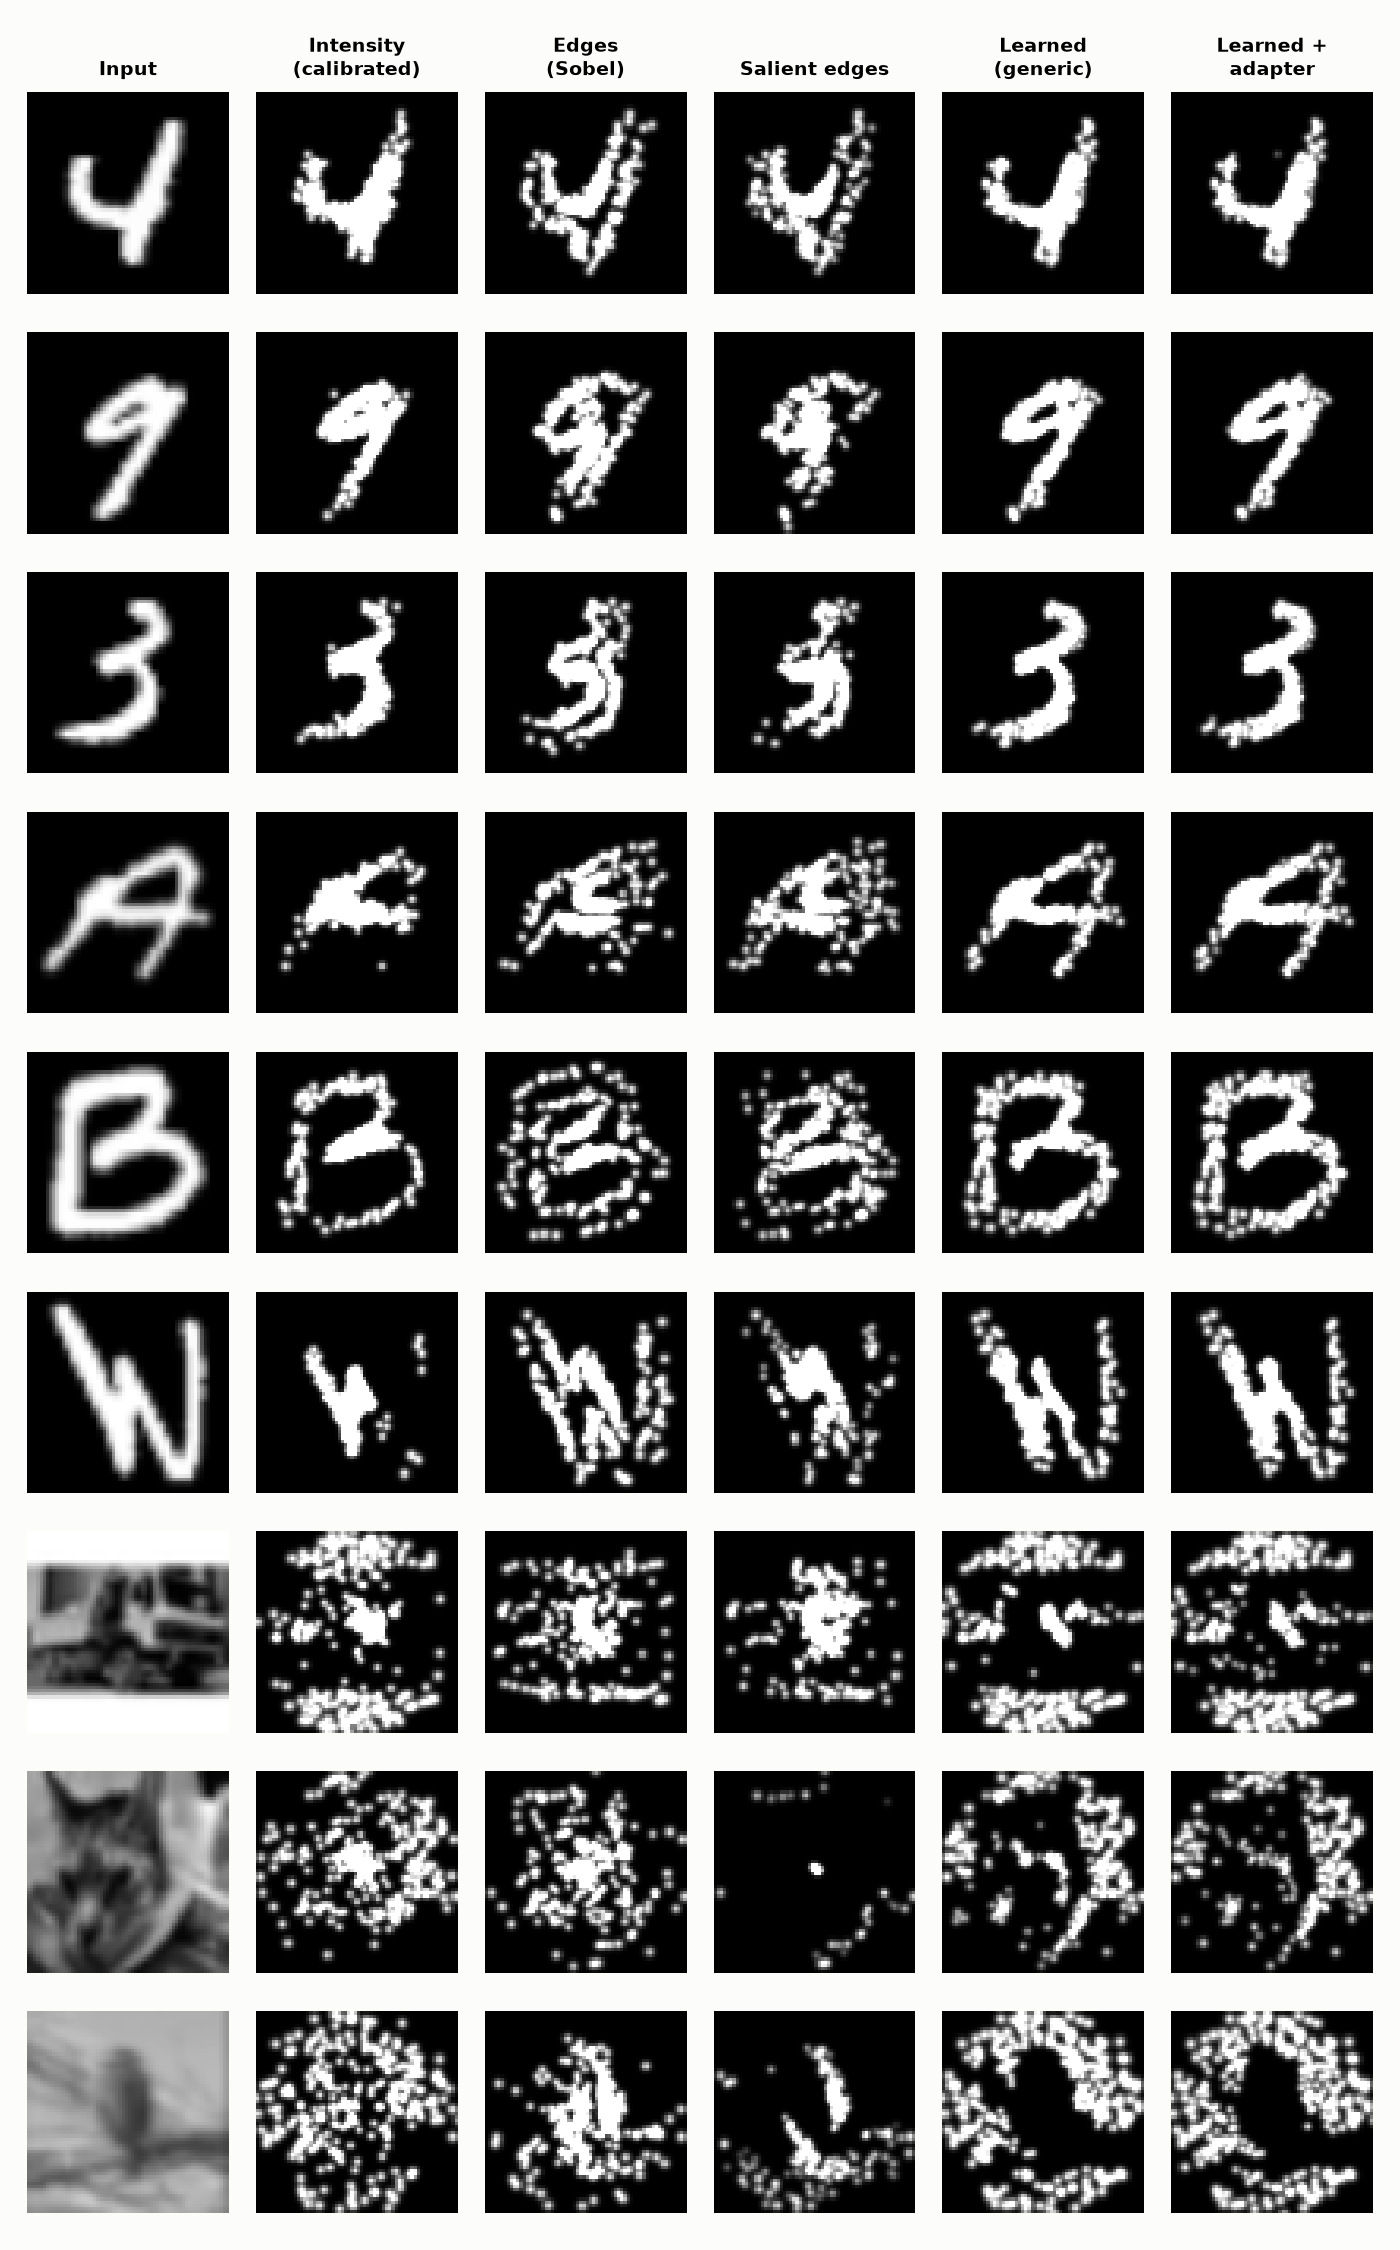
\includegraphics[width=\columnwidth]{fig_examples.png}
\caption{Example percepts on held-out patients for MNIST, EMNIST letters and CIFAR-10. With a 25\% active-electrode budget, intensity sampling can only light the 256 brightest sites, and drops parts of large shapes (e.g.\ the ``W''). The learned encoder spreads the same budget along the strokes.}
\label{fig:examples}
\end{figure}

\paragraph{Robustness to electrode failure.} Table~\ref{tab:dropout} and Fig.~\ref{fig:dropout} show performance after up to 50\% of the remaining electrodes fail without warning, with no recalibration and no classifier retraining:
\begin{itemize}
\item All encoders degrade gracefully up to 25\%.
\item At 50\% on MNIST and letters the learned encoder stays at or above the intensity baseline (\NumLettersLearnAccDropHalf\ against \NumLettersIntAccDropHalf\ on letters).
\item On CIFAR at 50\% it falls \emph{below} intensity sampling (\NumCifarLearnAccDropHalf\ against \NumCifarIntAccDropHalf).
\end{itemize}
Our reading of the CIFAR result is that the end-to-end encoder learns a distributed, texture-like code. That code is more informative when intact, but its percepts change more when half of it disappears, and the classifier was trained on intact percepts. Training-time electrode dropout beyond the 10\% in the training patients is the obvious fix, which we leave to the full-scale runs.

\GenDropoutTable

\begin{figure*}[t]
\centering
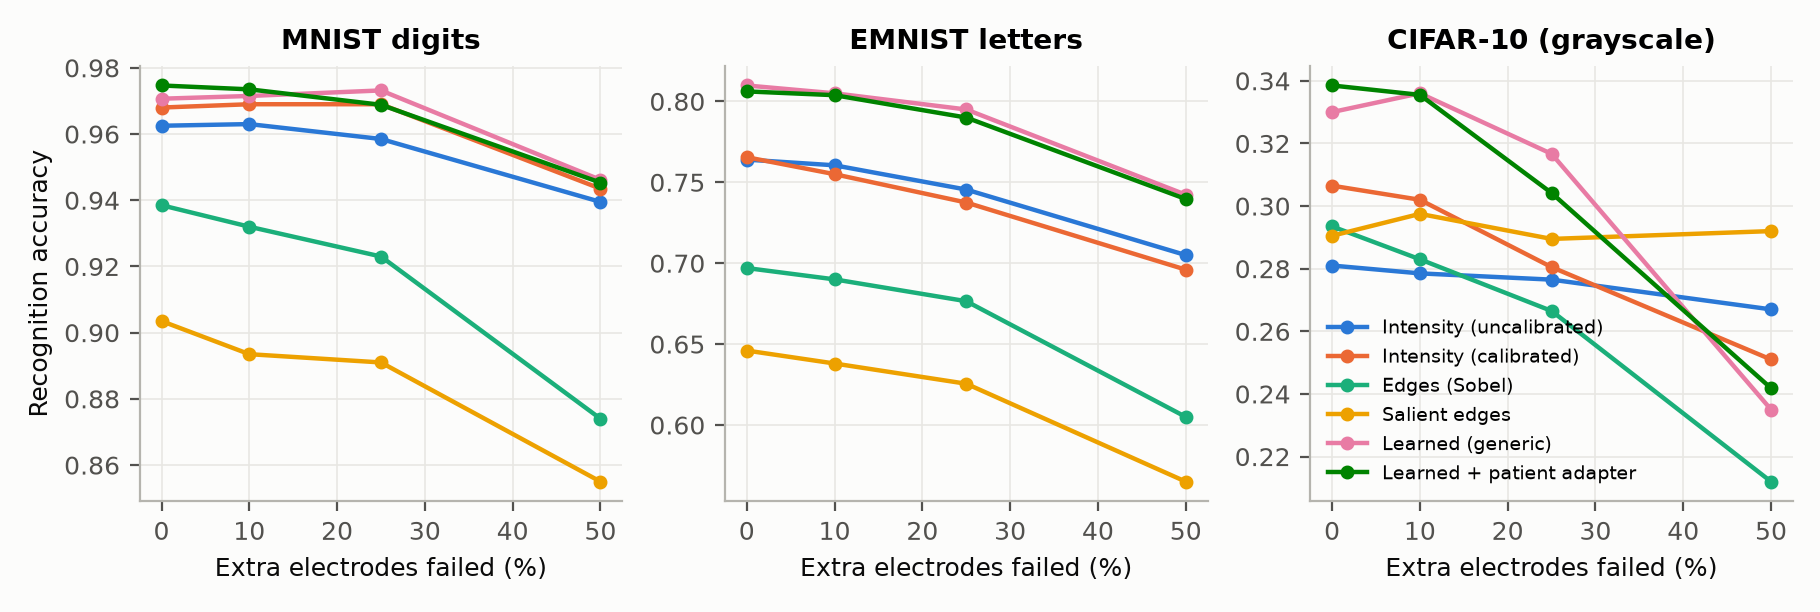
\includegraphics[width=\textwidth]{fig_dropout_robustness.png}
\caption{Recognition accuracy against the fraction of additional, unannounced electrode failures.}
\label{fig:dropout}
\end{figure*}
